\documentclass[10pt,a4paper]{article}
\usepackage[utf8]{inputenc}

\usepackage{amsmath}
\usepackage{amsfonts}
\usepackage{amssymb}
\usepackage{graphicx}
\usepackage{listings}
\usepackage{refstyle}


\lstset{numbers=left,
	title=\lstname,
	numberstyle=\tiny, 
	breaklines=true,
	tabsize=4,
	language=Python,
	morekeywords={with,super,as},,
	frame=single,
	basicstyle=\footnotesize\tt,
	commentstyle=\color{comment},
	keywordstyle=\color{keyword},
	stringstyle=\color{string},
	backgroundcolor=\color{white},
	showstringspaces=false,
	numbers=left,
	numbersep=5pt,
	literate=
		{æ}{{\ae}}1
		{å}{{\aa}}1
		{ø}{{\o}}1
		{Æ}{{\AE}}1
		{Å}{{\AA}}1
		{Ø}{{\O}}1
	}

\usepackage{bm}
\usepackage{hyperref}
\usepackage[margin=1.25 in]{geometry}
\usepackage[usenames, dvipsnames]{color}
\usepackage{float}
\usepackage{commath}

\begin{document}
\begin{center}


{\LARGE\bf
FYS4150\\
\vspace{0.5cm}
Project 3, deadline October 25.
}
 
\includegraphics[scale=0.075]{uio.png}\\
Author: Vemund Stenbekk Thorkildsen\\
\vspace{1cm}
{\LARGE\bf
Abstract
}\\
\end{center}
\newpage
{\LARGE\bf
Introduction
}\\
\noindent The Ising model in two dimensions will be studied and discussed in this report. The model is widely used, both in the study of phase transitions and statistics (source). In this report, the Ising model will be used to study phase transitions. In particular, the transition from a system with magnetic moment, to a system with zero magnetic moment. The Ising model predicts a phase shift at a given temperature. The system studied in this report will be a two dimensional lattice, where each lattice point only can take two different values. These values represent the spin, up-spin or down-spin, but can be represented in many ways. \\

\noindent The report will start off by an analytical solution for the case with a $2 \times 2$ lattice before moving on to solving this system numerically. This will be done by using the Metropolis algorithm. The results computed with the Metropolis algorithm will be compared to the analytic solutions. The main emphasis will be put on the Metropolis algorithm, its efficiency and precision (tror jeg).\\ 




{\LARGE\bf
Method
}\\

\noindent It is possible to derive an analytic solution for the simplest of the two dimensional case. Namely a $2 \times 2$ lattice with periodic boundary conditions. The partition dunction is given by:

\begin{equation}
Z= \sum\limits_{i=1}^{16}  e^{-J*E_{i}\beta}
\end{equation}

\noindent Where $\beta= \frac{1}{k_b T^2}$.  There are 16 different states of energy. Luckily, a lot of these yield the same result. Summing up all of these gives:

\begin{equation}
Z=2e^{-\beta 8 J}+2e^{\beta 8 J}+12
\end{equation}

\noindent The mean energy and magnetization is given by respectively:

\begin{equation}
E=\frac{1}{Z} \sum\limits_{i=1}^{16}  E_{i}e^{-J*E_{i}\beta}=\frac{-8e^{\beta 8J }+8e^{-\beta 8J}}{e^{-\beta 8 J}+e^{\beta 8 J}+6}
\end{equation}
and
\begin{equation}
M=\frac{1}{Z}\sum\limits_{i=1}^{16}  M_{i}e^{-J*E_{i}\beta}=\frac{4e^{\beta 8J}+8}{e^{-\beta 8 J}+e^{\beta 8 J}+6}
\end{equation}

\noindent The specific heat is given as the variance of energy divided by $k_b T^2$:

\begin{equation} 
c_v =\frac{64}{k_b T} \frac{1+3cosh(8\beta)}{(cosh(8\beta)+3)^2}
\end{equation}

\noindent The variance of magnetism divided by $k_b T$ reveals the susceptibility.

\begin{equation}
X=\frac{1}{k_b T} \Bigg(\frac{32^{\frac{8}{k_b T}}+32}{Z} - \Big(\frac{8e^{\frac{8}{k_b T}}+16}{Z}\Big)^2\Bigg)
\end{equation}

\noindent This problem will be solved by using the metropolis algorithm. 












 





\newpage
{\LARGE\bf
Results
}

\noindent The $2\times2$ matrix will serve as a benchmark to test the program in this report. This can be done as the analytic equations can be derived for this simple case.\\ 

\textbf{Table 1:} Mean energy and specific heat for $T=1.0$ \\
\centerline{
\begin{tabular}{c|c|c|c|c}
\hline
Monte Carlo cycles & Mean E random matrix & Mean E up matrix & $C_v$ random matrix & $C_v$ up matrix\\
\hline
$10^1$ & -8 & -8 & 0 & 0 \\
\hline
$10^2$ & -7.92079 & -8 &  0.627389 & 0 \\
\hline
$10^3$ &  -7.97602 & -7.97602 &  0.191233 & 0.0638722 \\
\hline
$10^4$ & -7.9808 & -7.984 &  0.121357 & 0.108604\\
\hline
$10^5$ & -7.98952 & -7.98424 & 0.13093 &  0.118817 \\
\hline
$10^6$ & -7.9836 & -7.98339 & 0.127234 & 0.128955 \\
\hline
Numerical & -7.9839 & -7.9839 & 0.1282 & 0.1282\\
\hline
\end{tabular}
}
\noindent The Mean energy moves quickly towards the analytic result. The mean is in fact accurate up to three leading digits even for $10^4$ monte carlo cycles for both a random matrix and a all up initial matrix. The specific heat in this case is the same as the variance ($C_v=\frac{Variance}{k_b T^2}$ with $ k_b T^2=1$)This property is more sensitive, and it is needed $10^6$ monte carlo cycles before reaching an accuracy of two leading digits for the random matrix, and three leading digits for the all up initial matrix. The results varied when running the program, which is to be expected for a probability influenced system. \\

\textbf{Table 2:} Mean absolute value of the magnetization and susceptibility for $T=1.0$\\
\centerline{
\begin{tabular}{c|c|c|c|c}
\hline
Monte Carlo cycles & Mean \abs{M} random matrix & Mean \abs{M} up matrix & $X$ random matrix & $X$ up matrix\\
\hline
$10^1$ & 4 & 4 & 0 & 0\\
\hline
$10^2$ & 3.94059 &3.9604 & 0.115283 & 0.156847\\
\hline
$10^3$ & 3.998 & 3.99401 & 0.00399201 & 0.0199441 \\
\hline
$10^4$ & 3.9952 & 3.9924 & 0.0127757 & 0.0239399 \\
\hline
$10^5$ & 3.99382 & 3.99396 & 0.0178416 & 0.0188433 \\
\hline
$10^6$ & 3.99456 & 3.9949 & 0.0164823 & 0.0150619 \\
\hline
Numerical & 3.9946 & 3.9946 & 0.0160 &0.0160\\
\hline
\end{tabular}
}
The results for magnetization and susceptibility tell much of the same story. The mean absolute value of the magnetization is accurate with three leading digits for  $10^3$ monte carlo cycles in both the random and all up case. As for the specific heat, the susceptibility is here equal to the variance of magnetism. The susceptibility is not stable before being computed with $10^6$ Monte Carlo cycles, and even then it is not accurate over two or one leading digits.


  
\newpage
all figures of energy and magnetization were plotted with 1 000 000 monte carlo cycles and written to file for every 2500 points 


\begin{figure} [H]
\centerline{
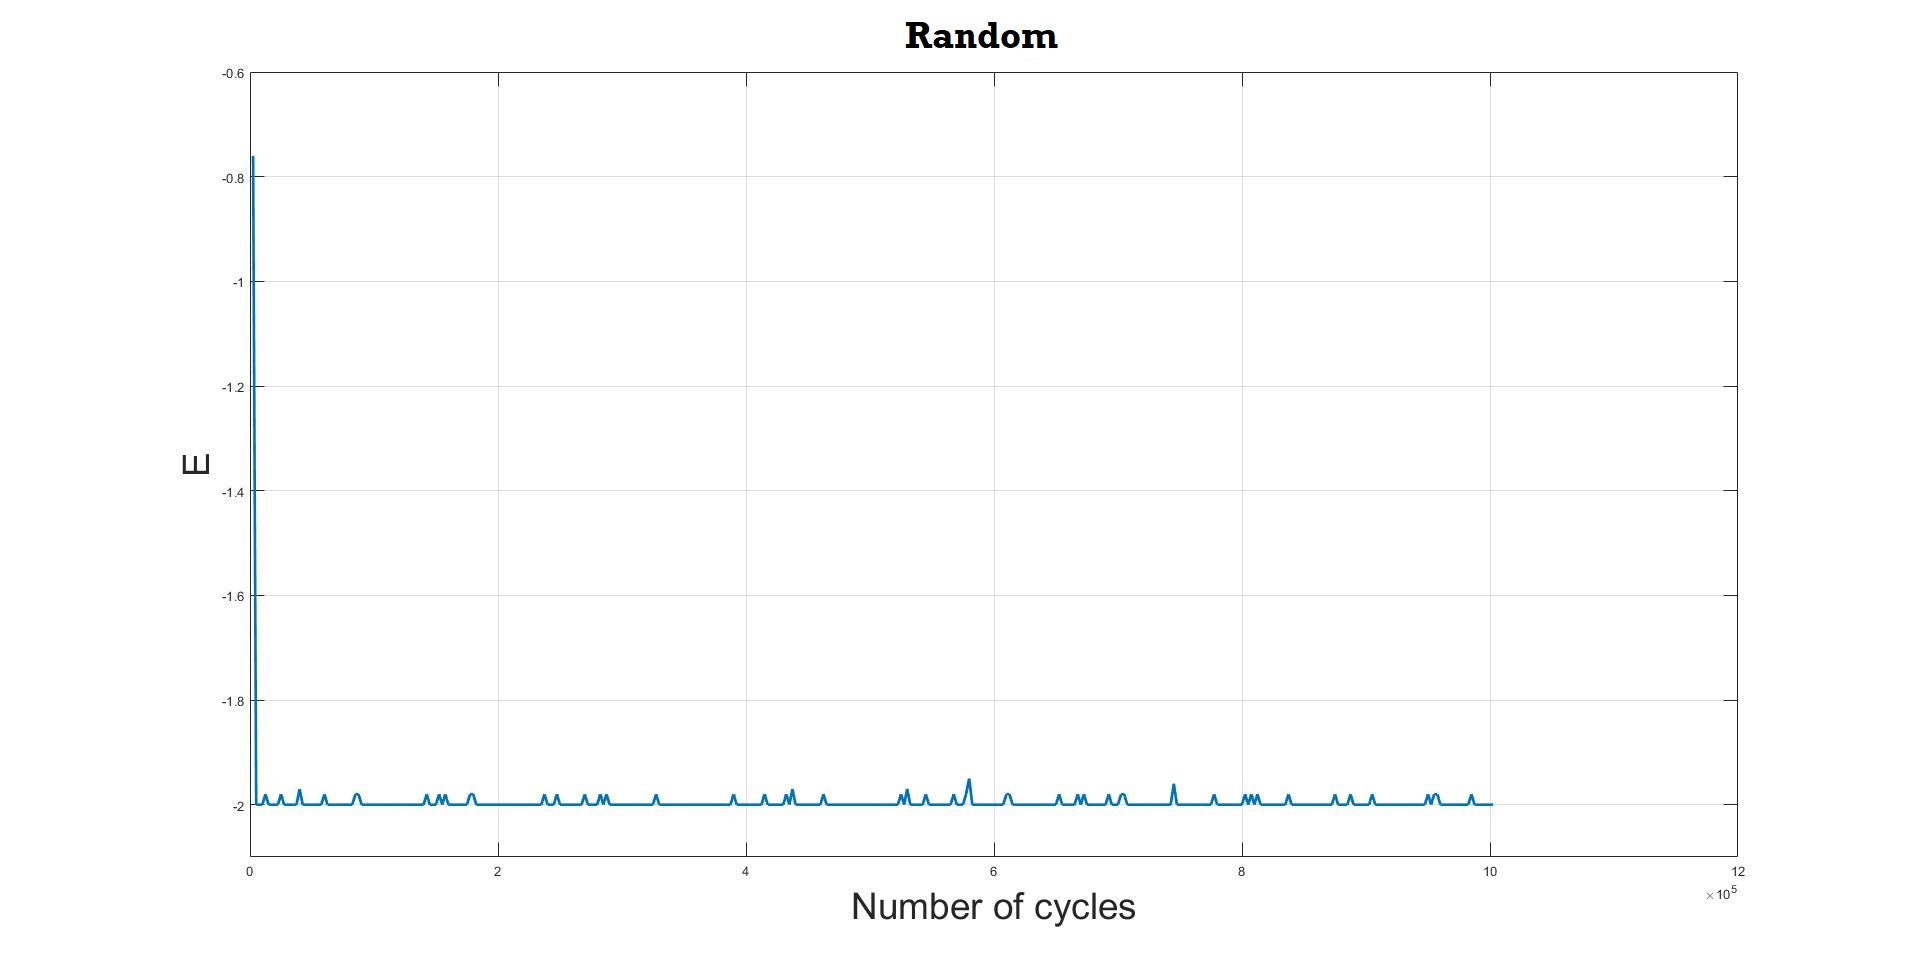
\includegraphics[scale=0.15]{RANDOMenergy1.jpg}
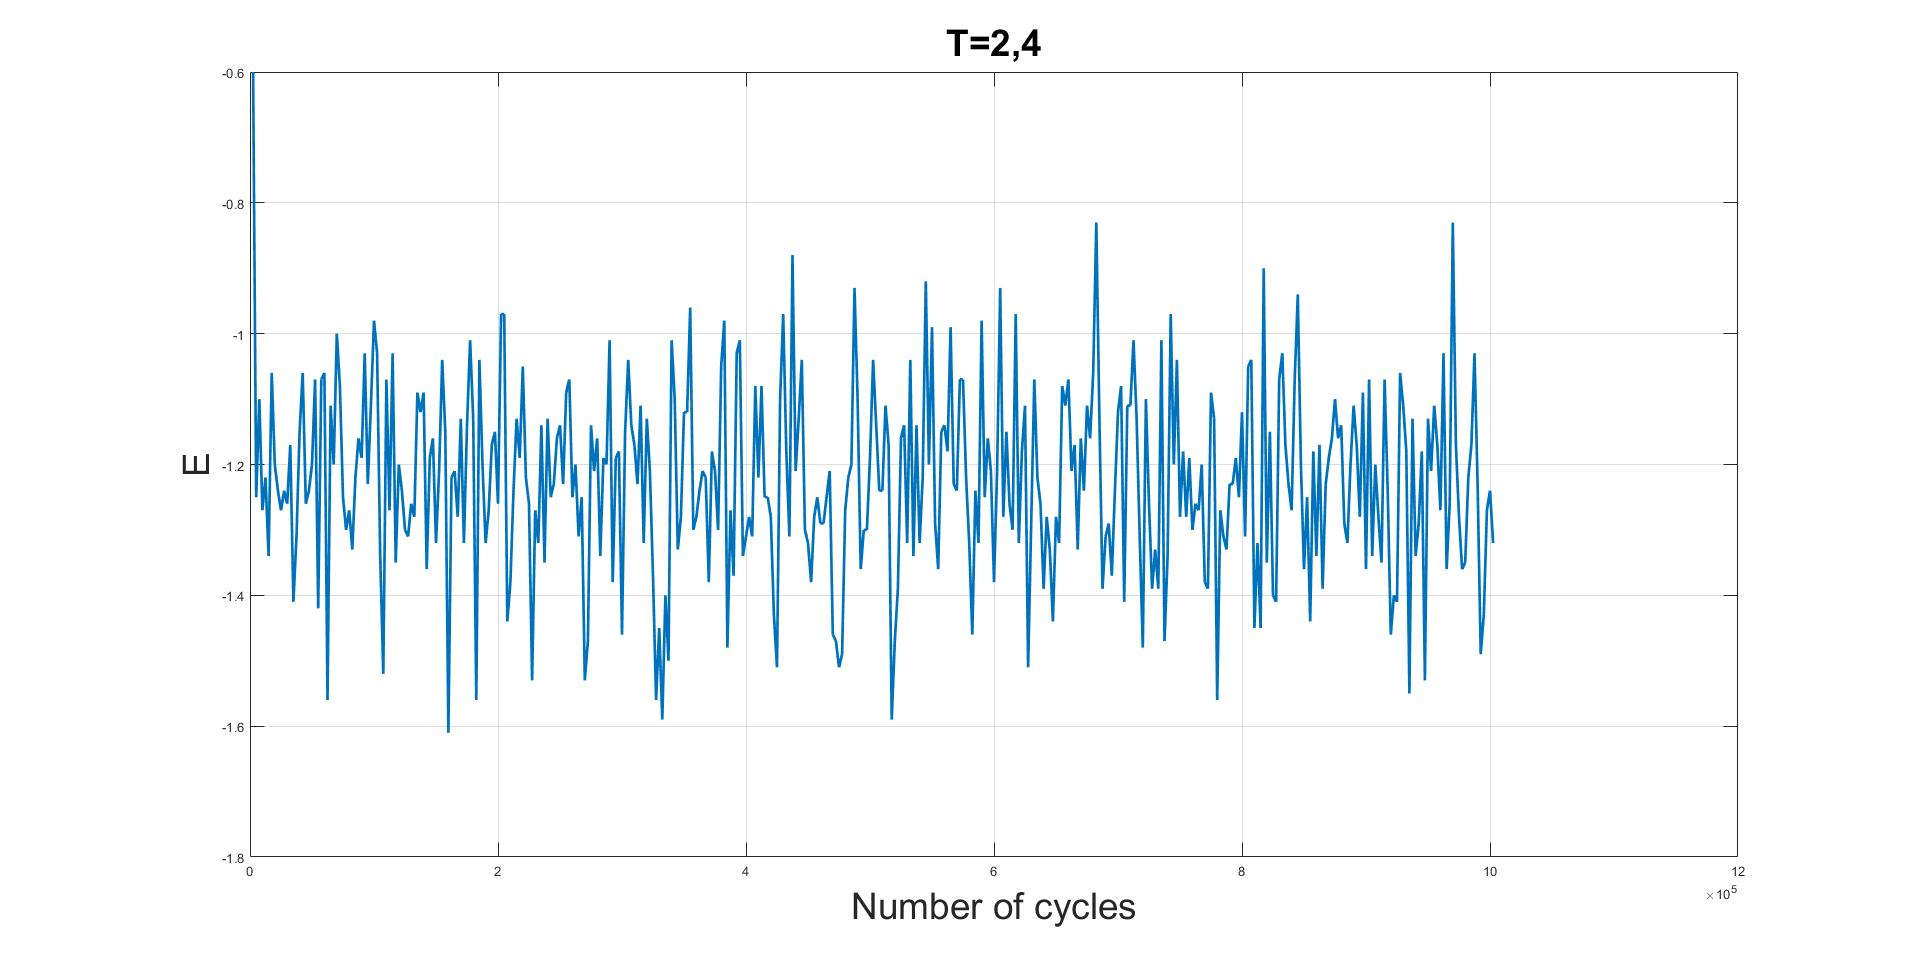
\includegraphics[scale=0.15]{RANDOMenergy24.jpg}
}
\caption{Energy of random initial matrix per lattice point plotted against number of monte carlo cycles for T=1.0 and T=2.4}
\label{fig:RandomEnergy}
\end{figure}


\begin{figure} [H]
\centerline{
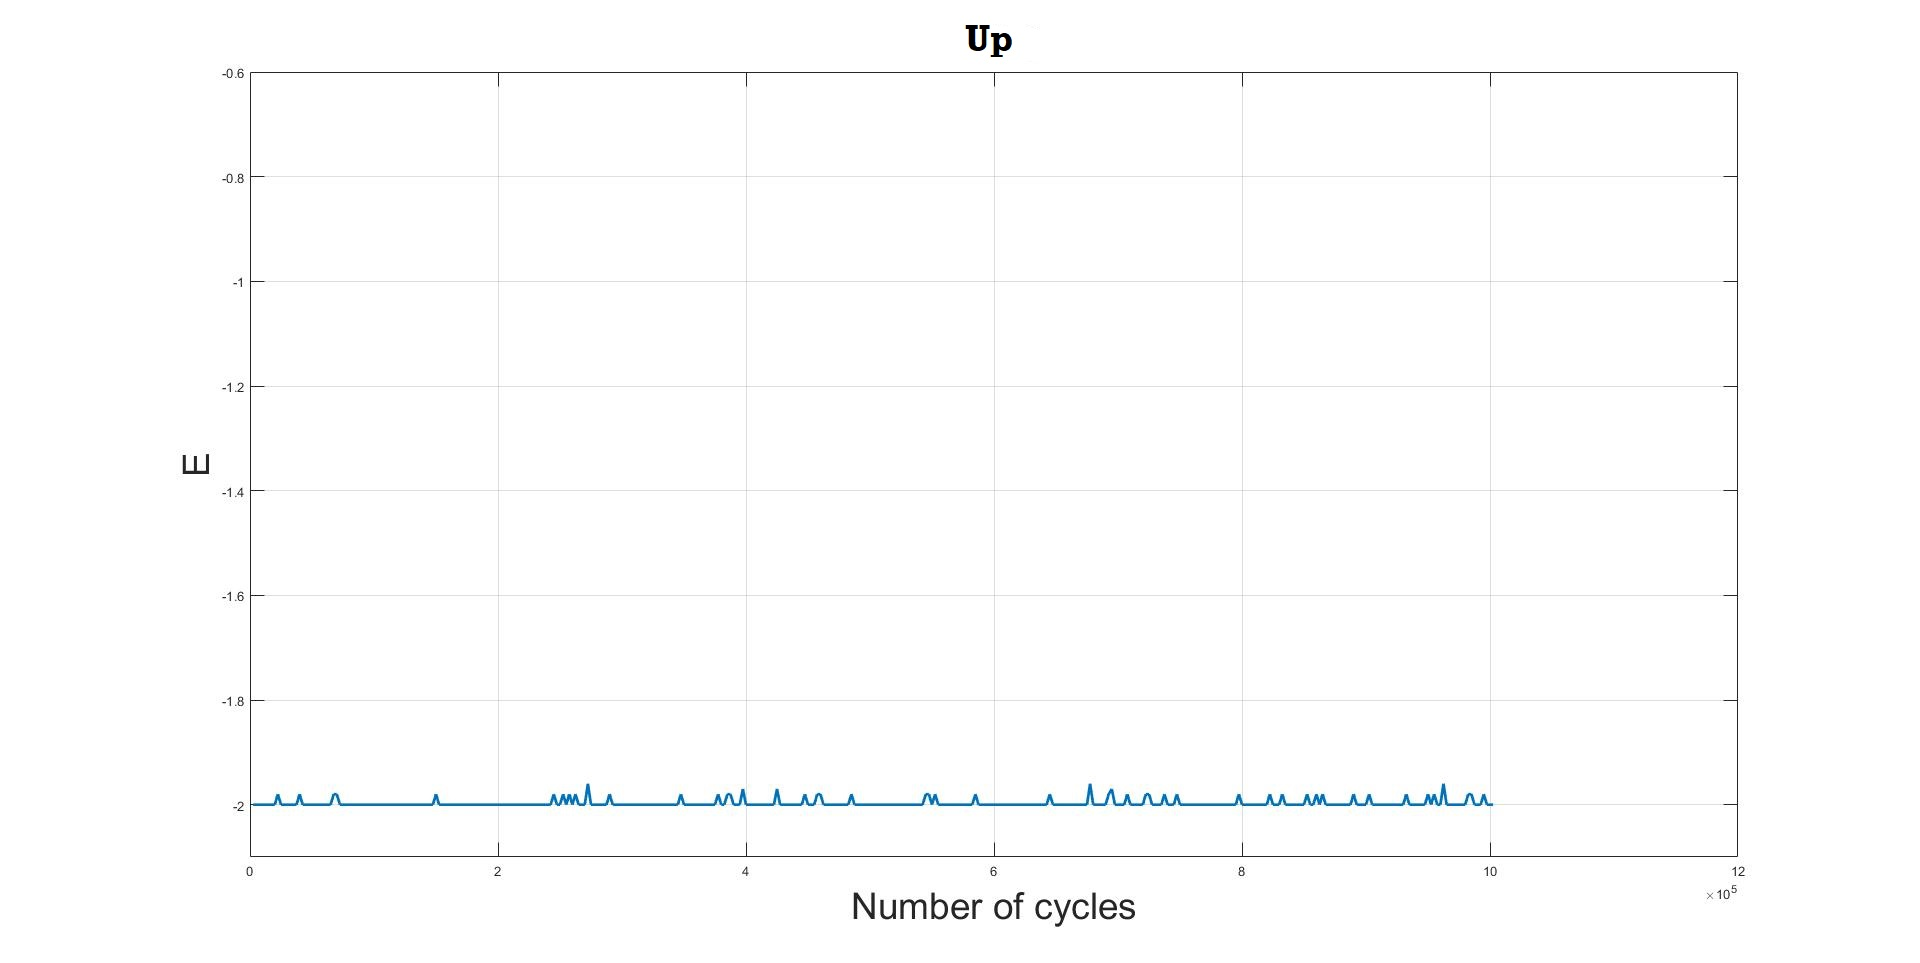
\includegraphics[scale=0.15]{UPenergy1.jpg}
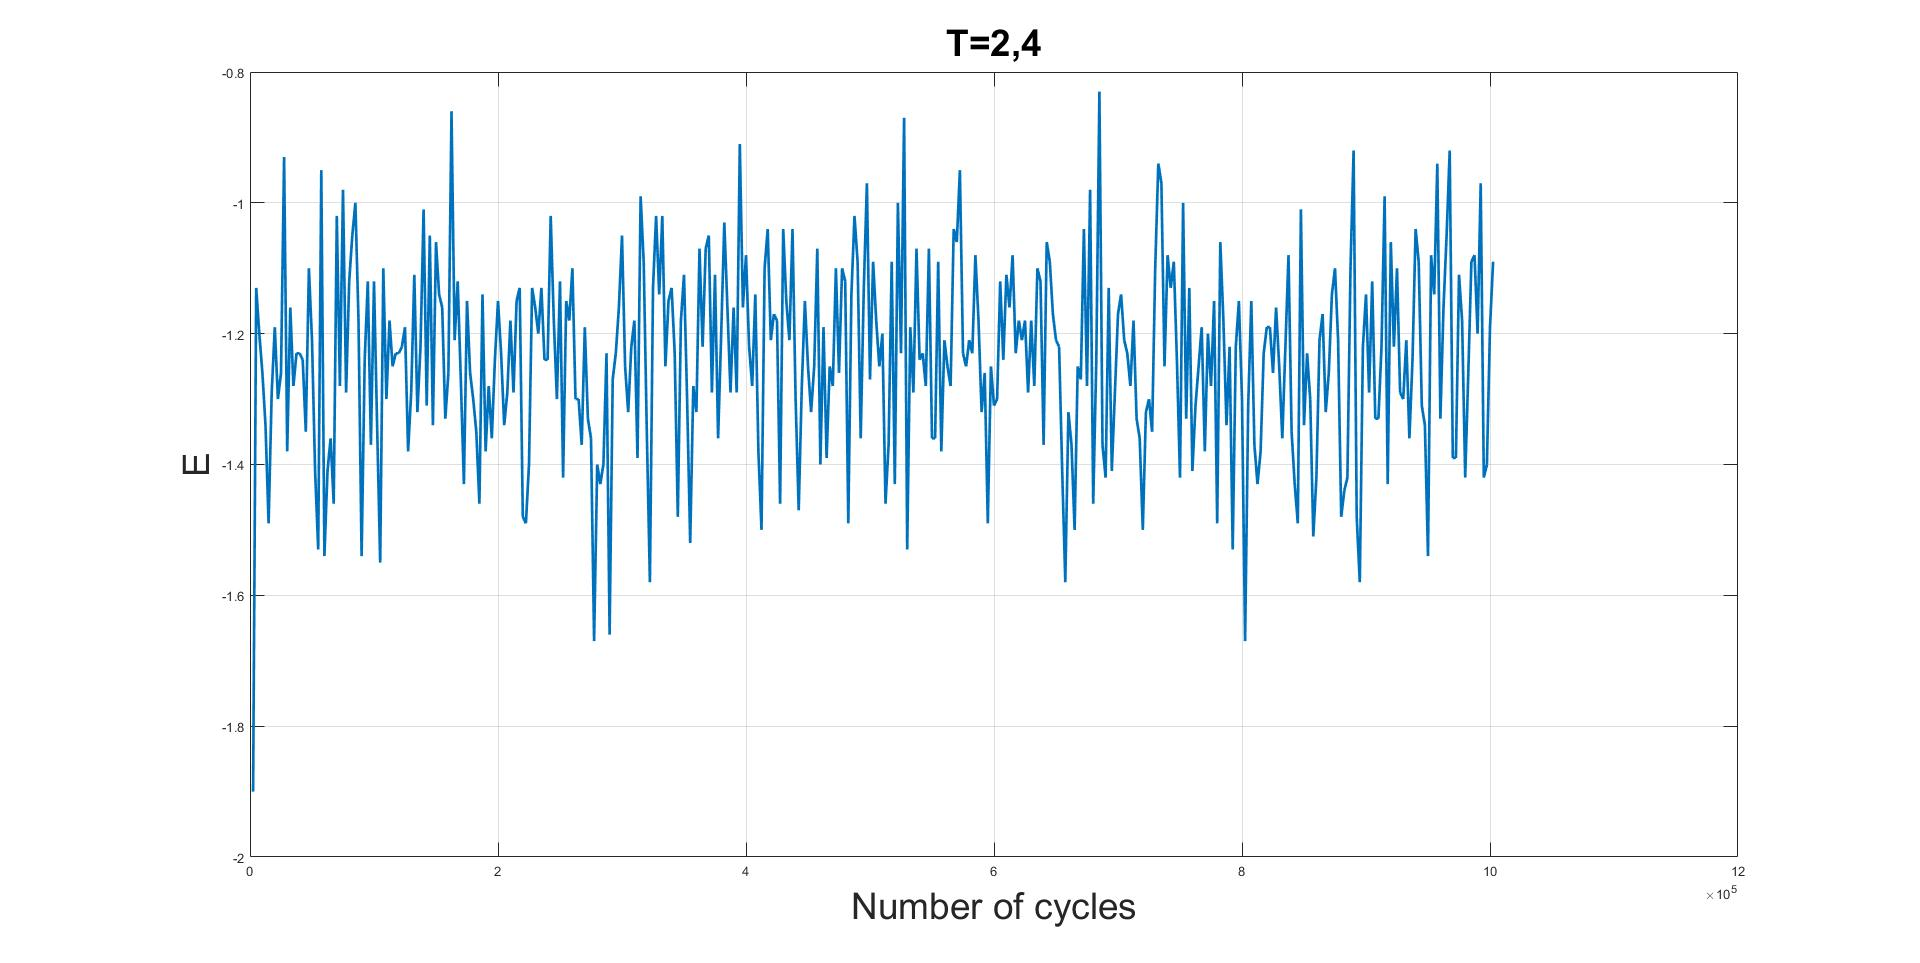
\includegraphics[scale=0.15]{UPenergy24.jpg}
}
\caption{Energy of all spins up initital matrix plotted against number of monte carlo cycles}
\label{fig:UpEnergy}
\end{figure}

\noindent It is clear to see in \figref{RandomEnergy} and \figref{UpEnergy} that the energy quickly converges to a steady state around $-2$ when $T=1.0$. For the all up initial configuration, it is already at this steady state. This equilibrium state is confined to a small number of energy levels. For $T=2.4$ the energy also converges to an equilibrium state, but the energy fluctuates more than for lower temperature. This is to be expected, because there is more energy in the system, and will be elaborated further later in the report. 

\begin{figure} [H]
\centerline{
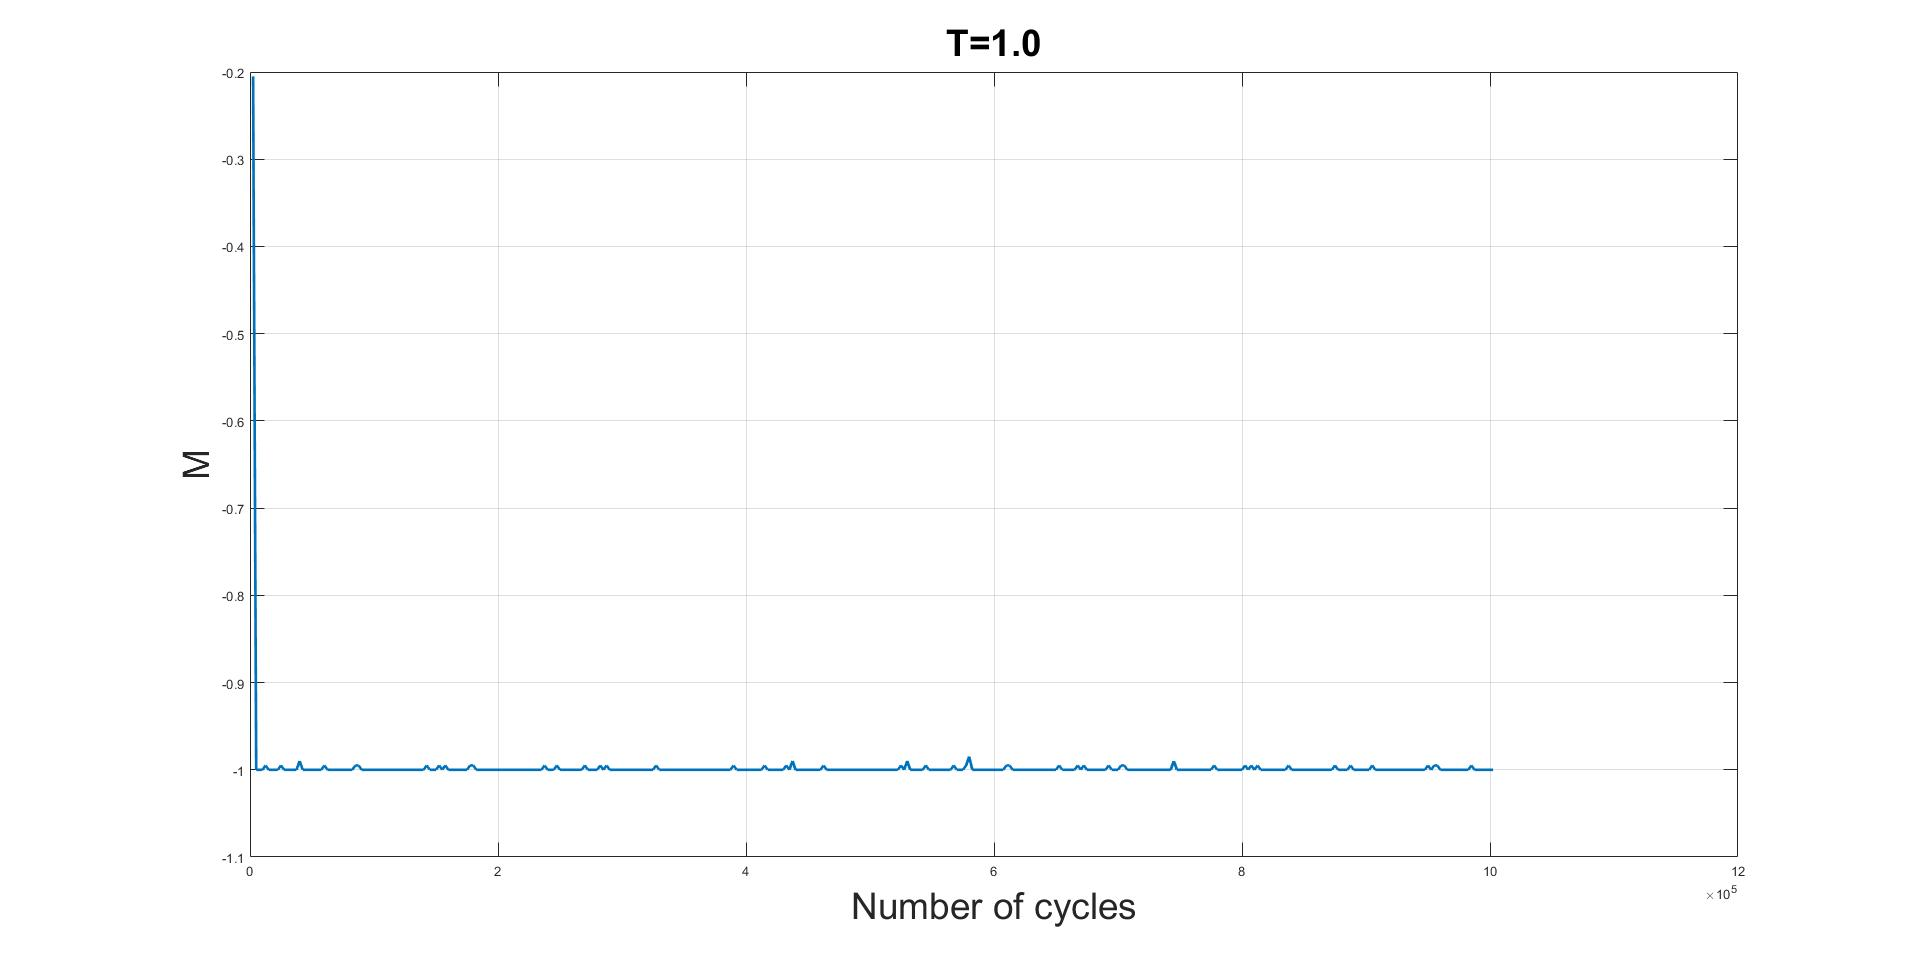
\includegraphics[scale=0.15]{RANDOMmag1notabs.jpg}
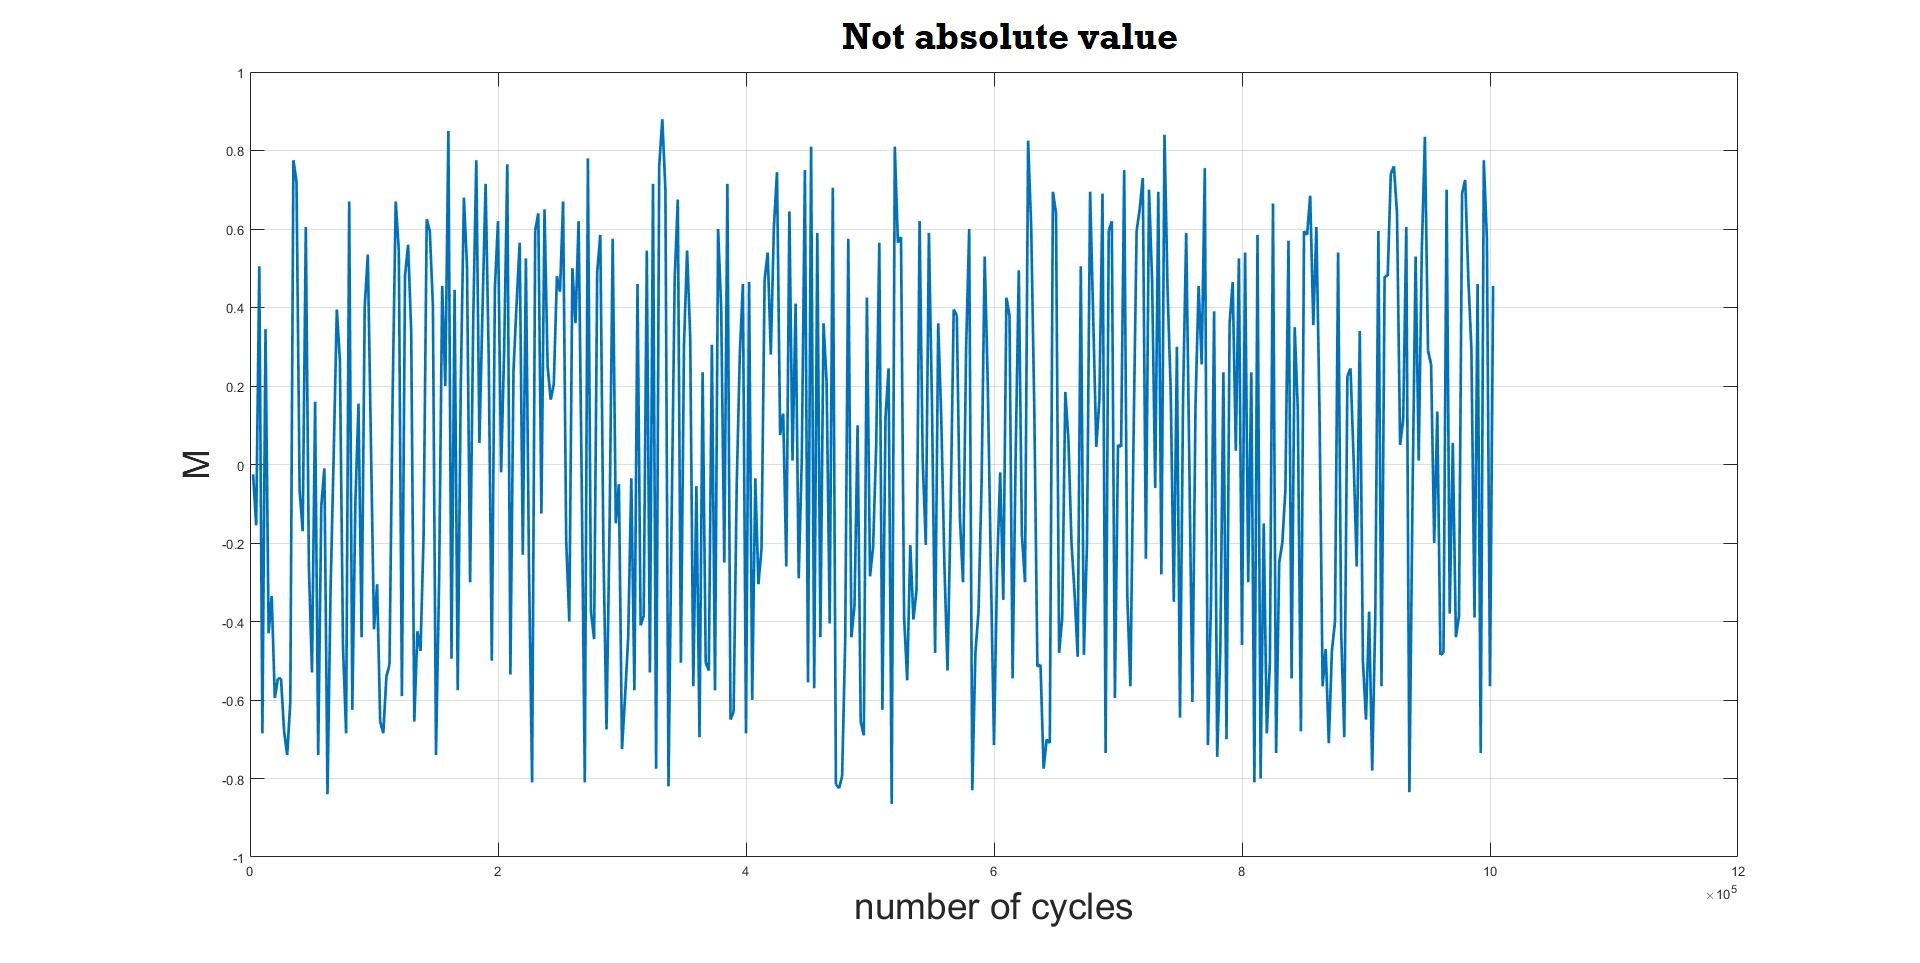
\includegraphics[scale=0.15]{RANDOMmag24notabs.jpg}
}
\caption{Random starting matrices magnetization not absolute value}
\label{fig:RandomMagNotAbs}
\end{figure}


\begin{figure}
\centerline{
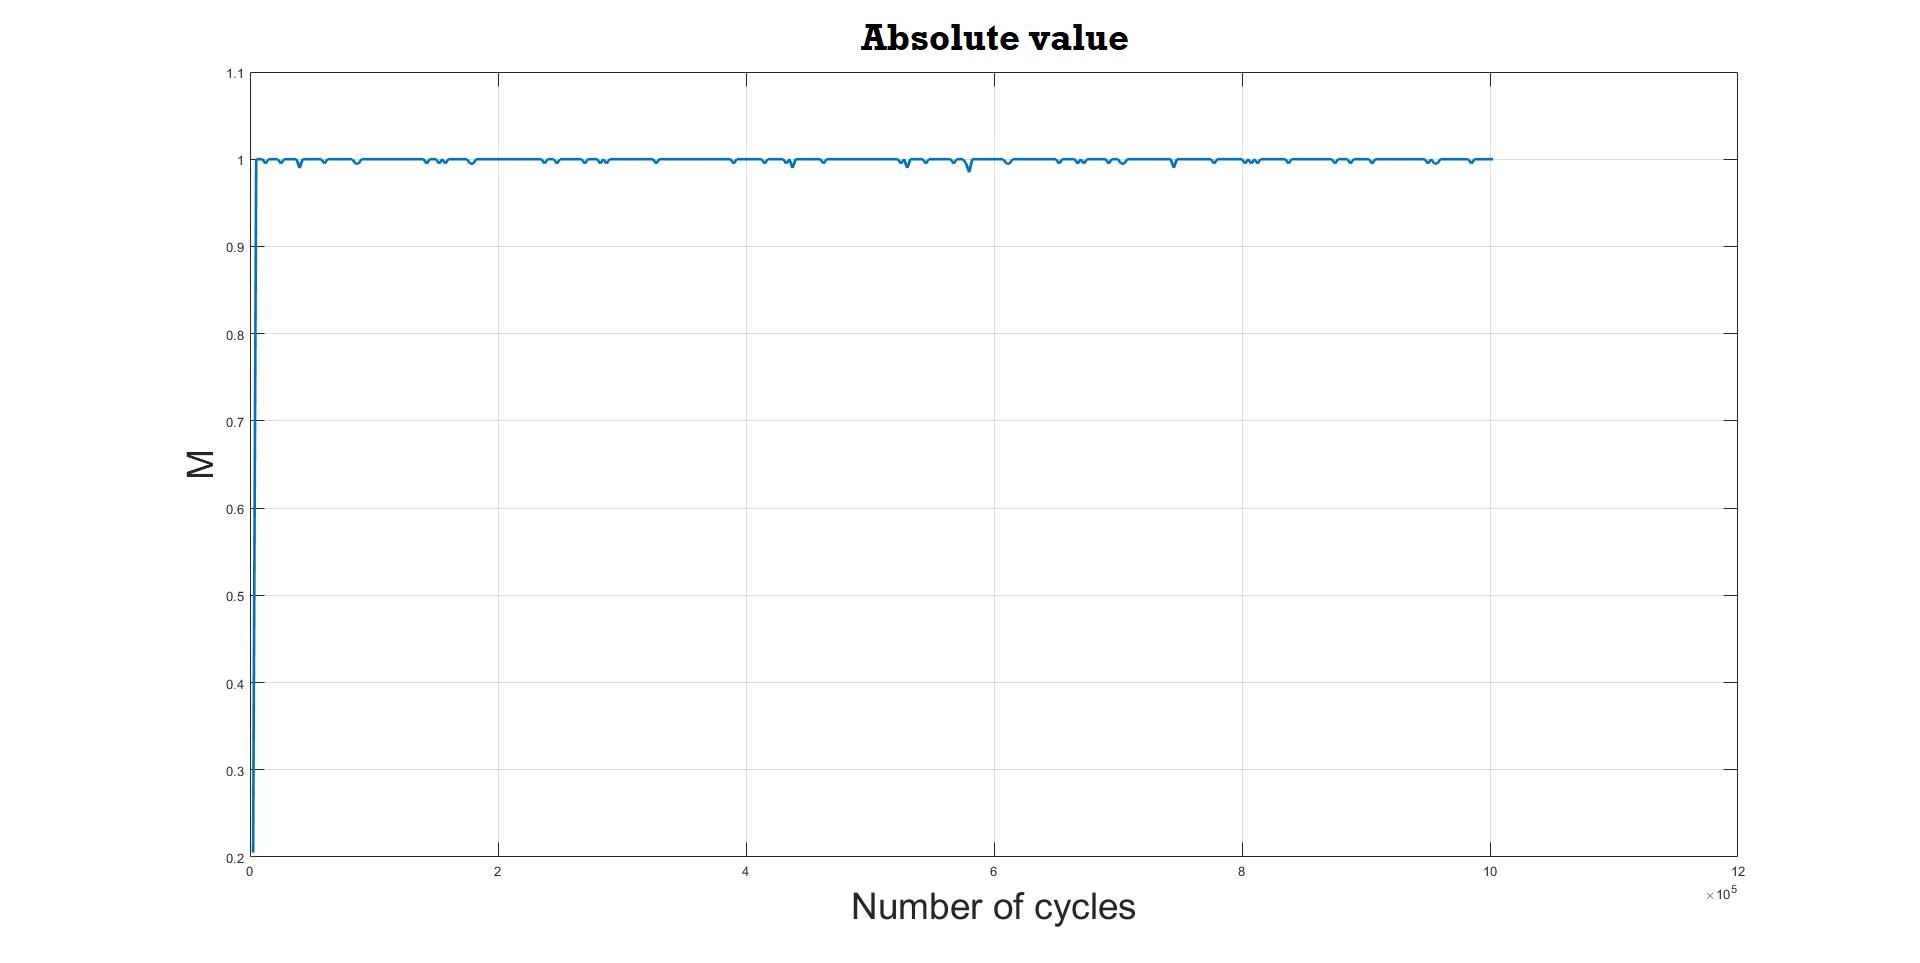
\includegraphics[scale=0.15]{RANDOMmag1abs.jpg}
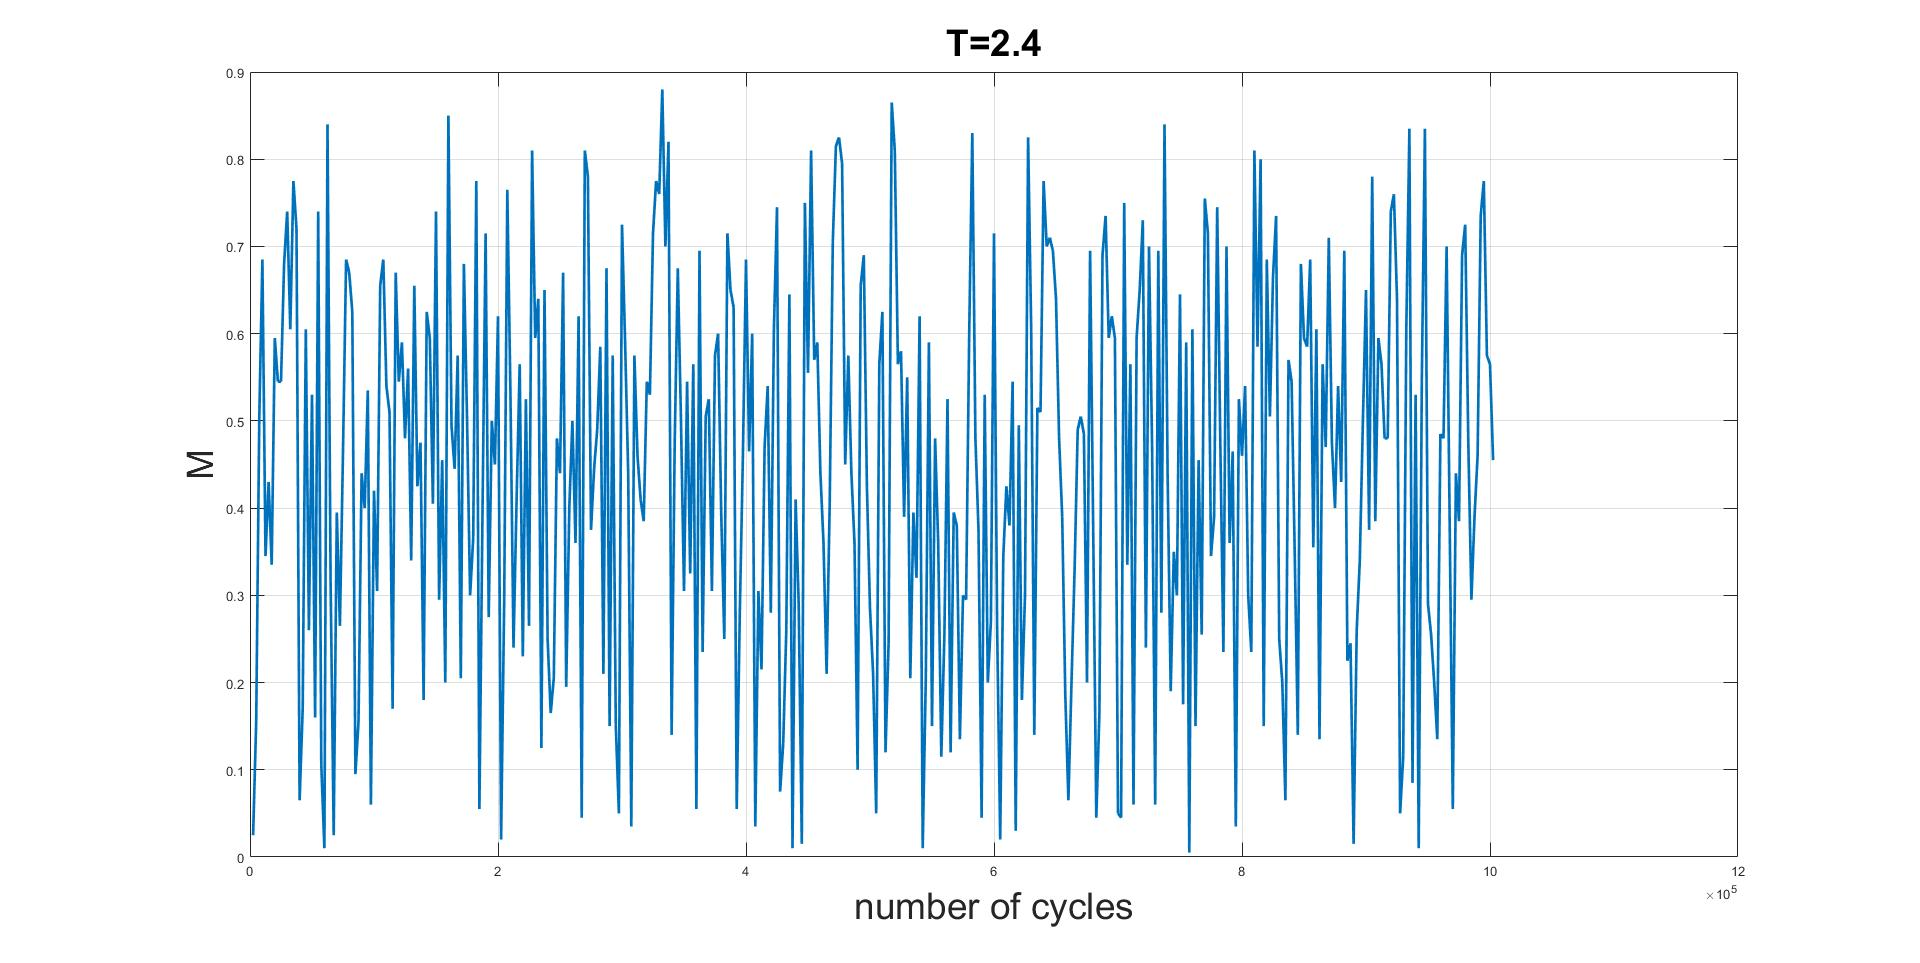
\includegraphics[scale=0.15]{RANDOMmag24abs.jpg}
}
\caption{Random starting matrices magnetization with absolute value }
\label{fig:RandomMagAbs}
\end{figure}

\begin{figure} [H]
\centerline{
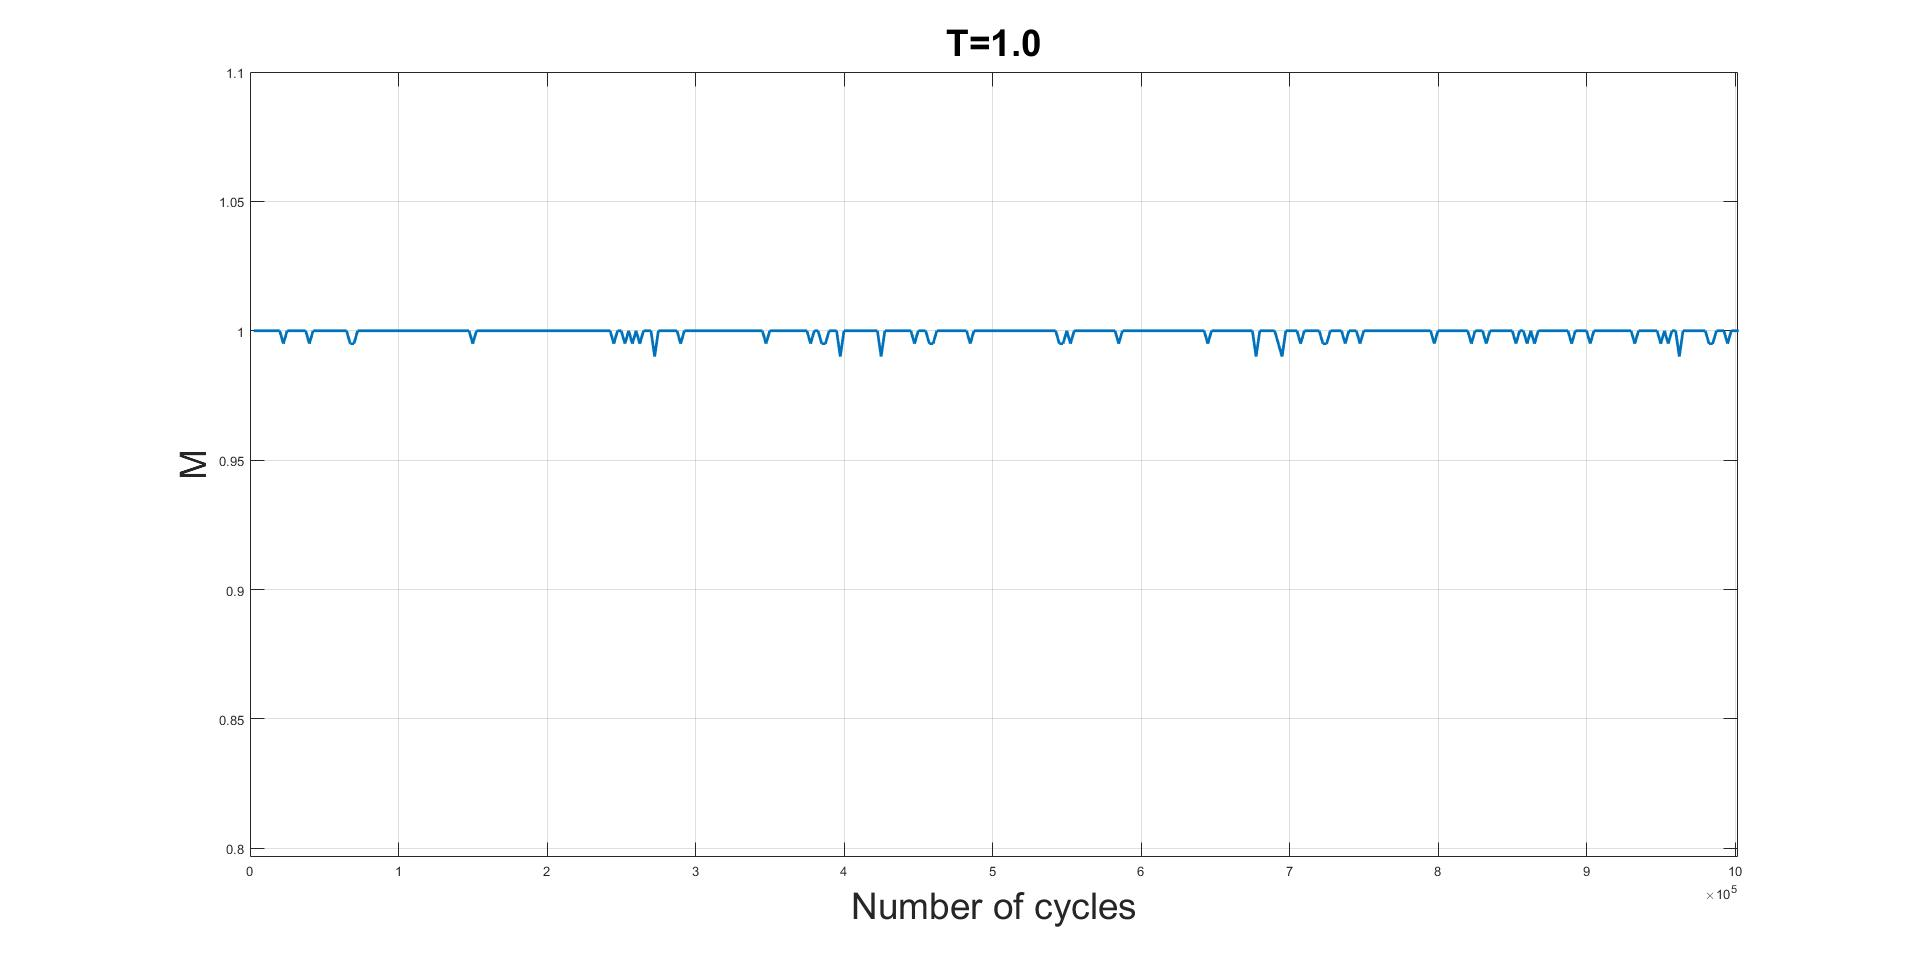
\includegraphics[scale=0.15]{UPmag1notabs.jpg}
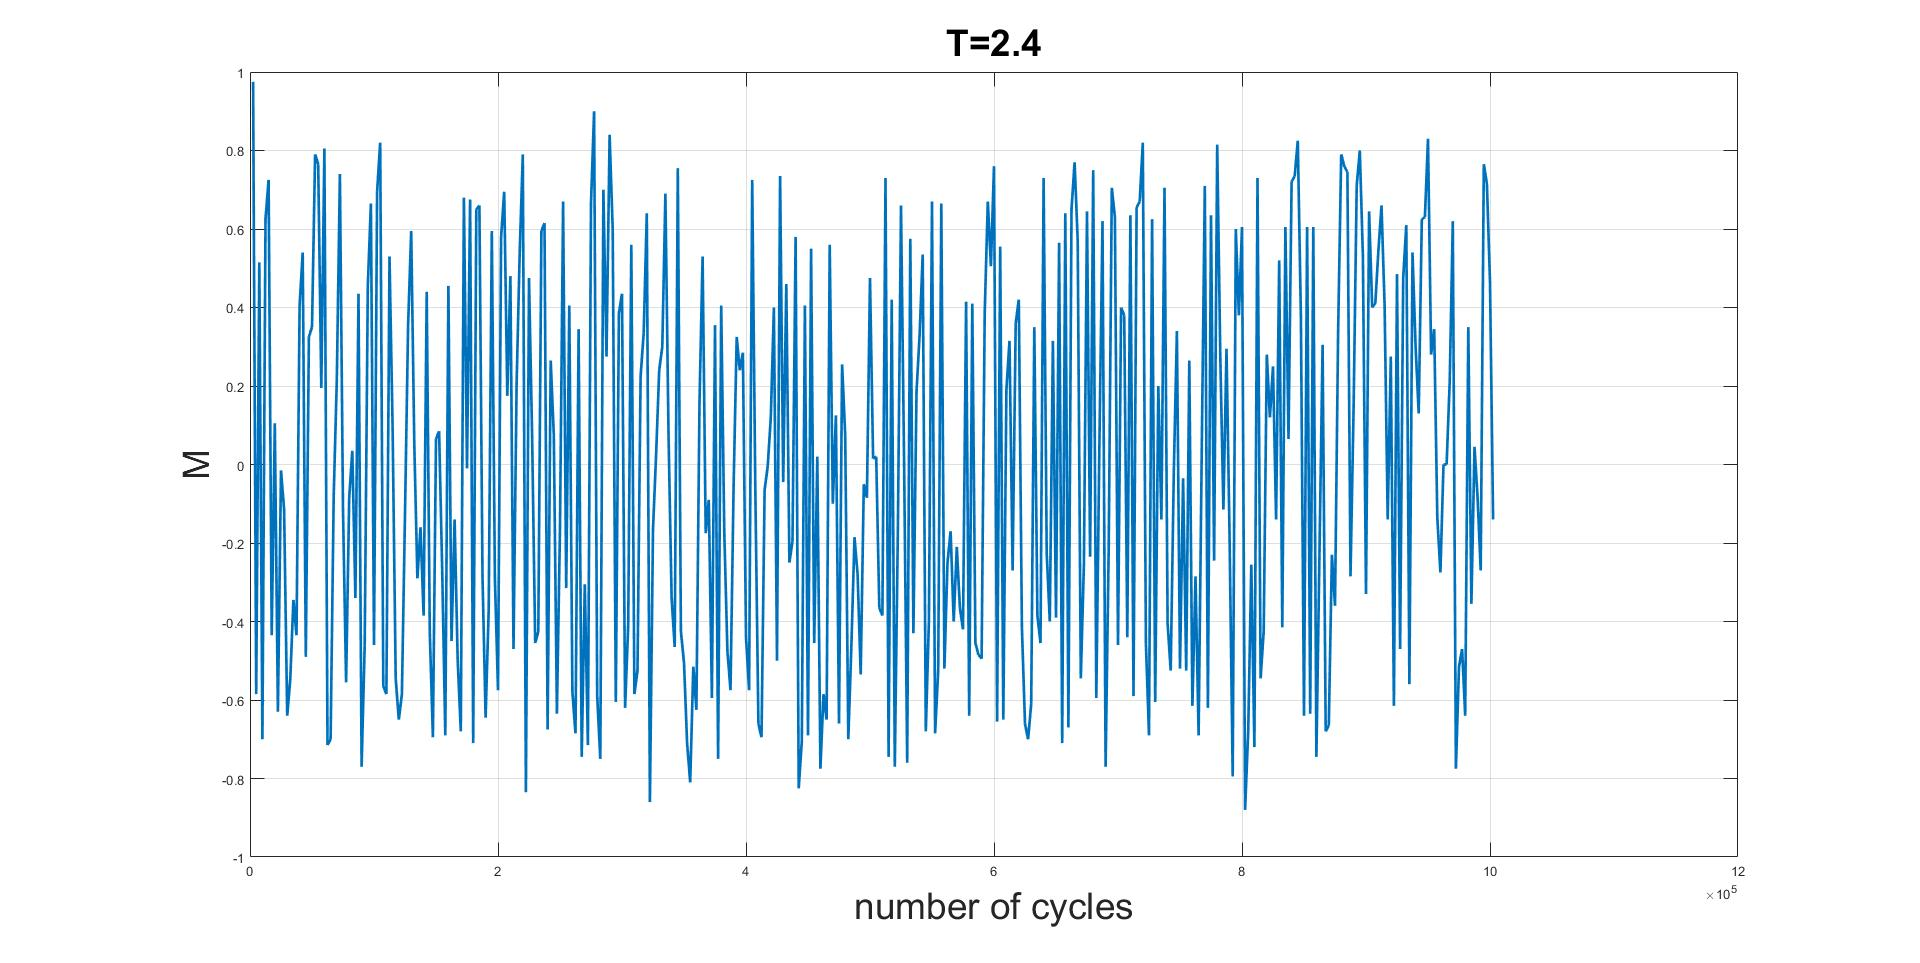
\includegraphics[scale=0.15]{UPmag24notabs.jpg}
}
\caption{All up starting matrices, magnetism not absolute value}
\label{fig:UpMagNotAbs}
\end{figure}


\begin{figure}
\centerline{
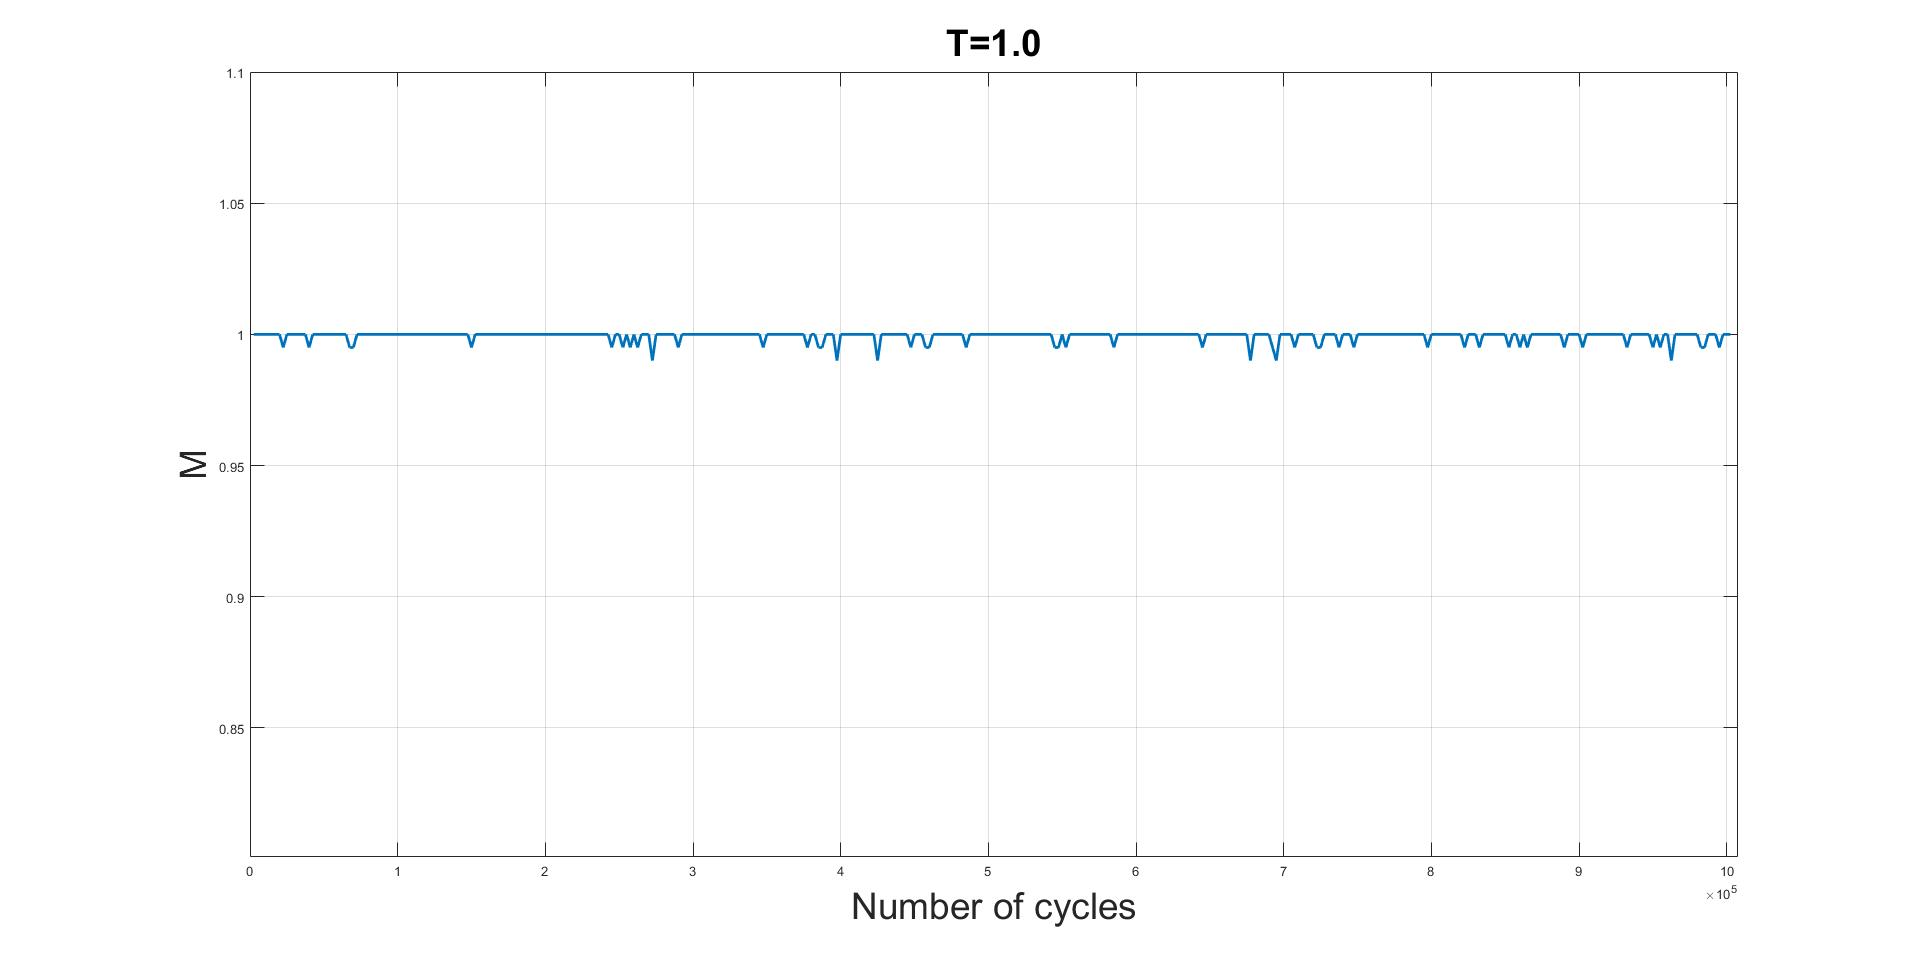
\includegraphics[scale=0.15]{UPmag1abs.jpg}
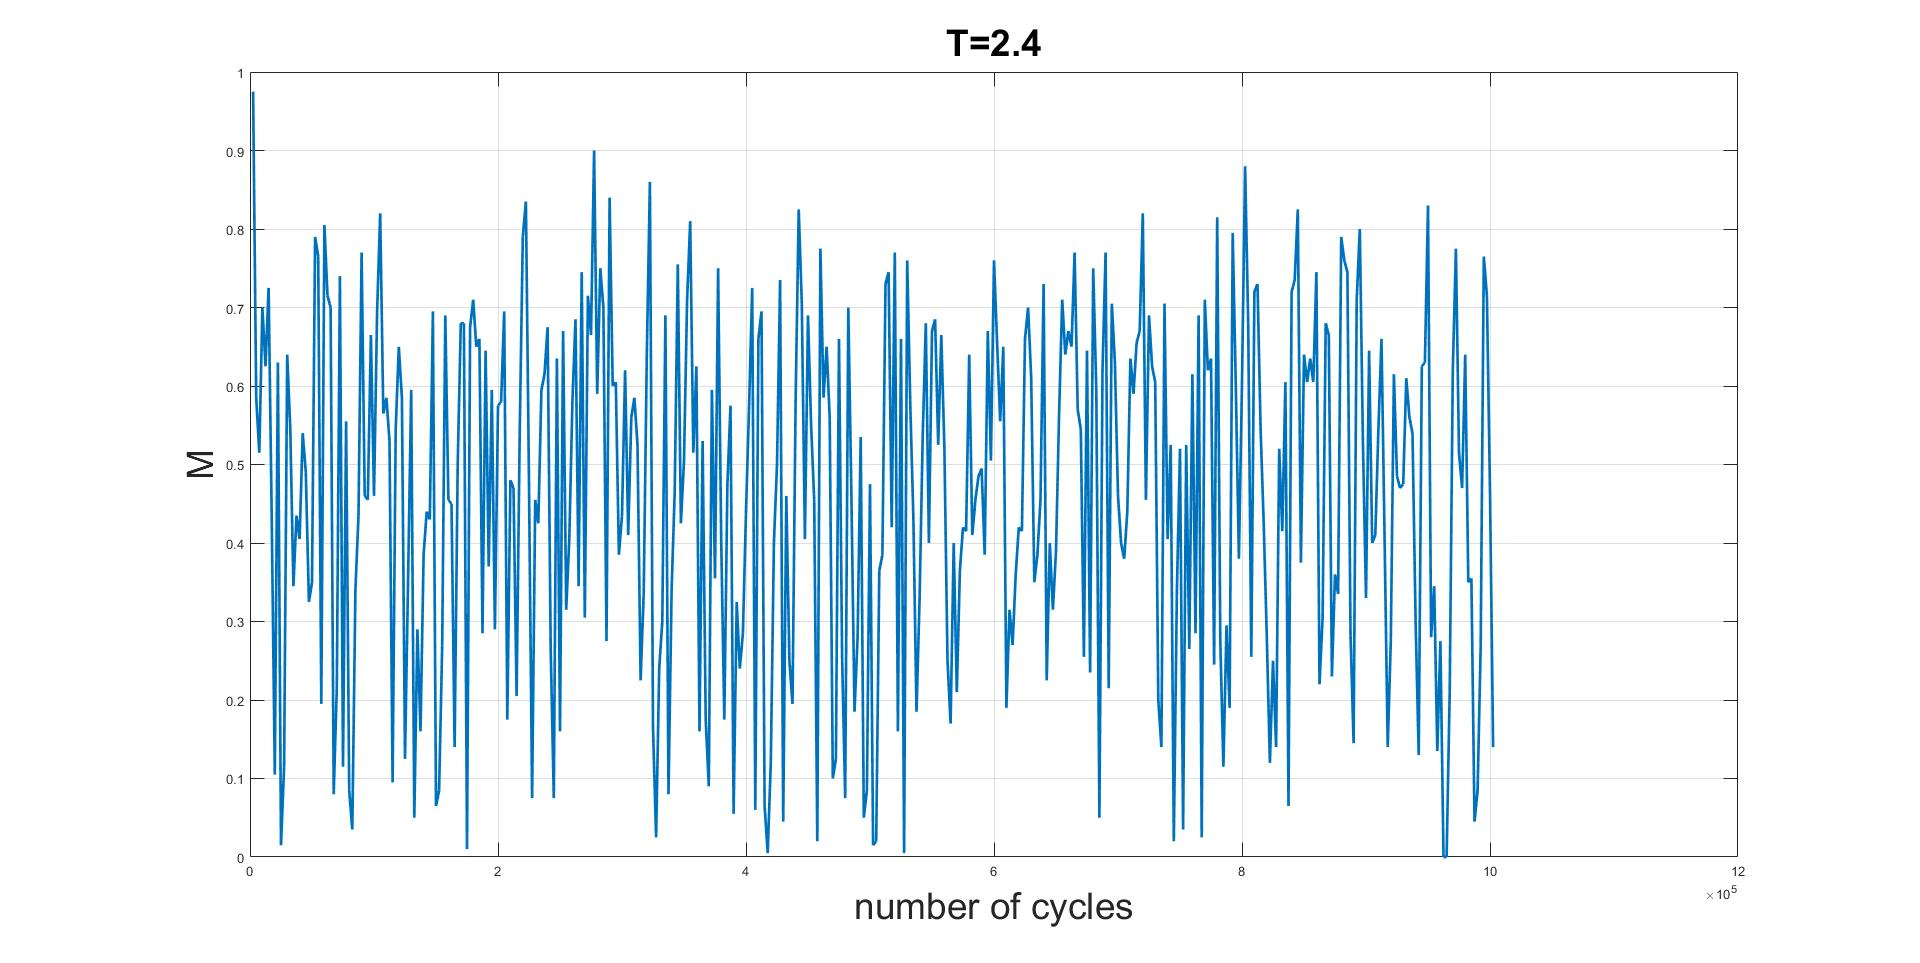
\includegraphics[scale=0.15]{UPmag24abs.jpg}
}
\caption{All up starting matrices, magnetism absolute value}
\label{fig:UpMagnetizm}
\end{figure}


\begin{figure} [H]
\centerline{
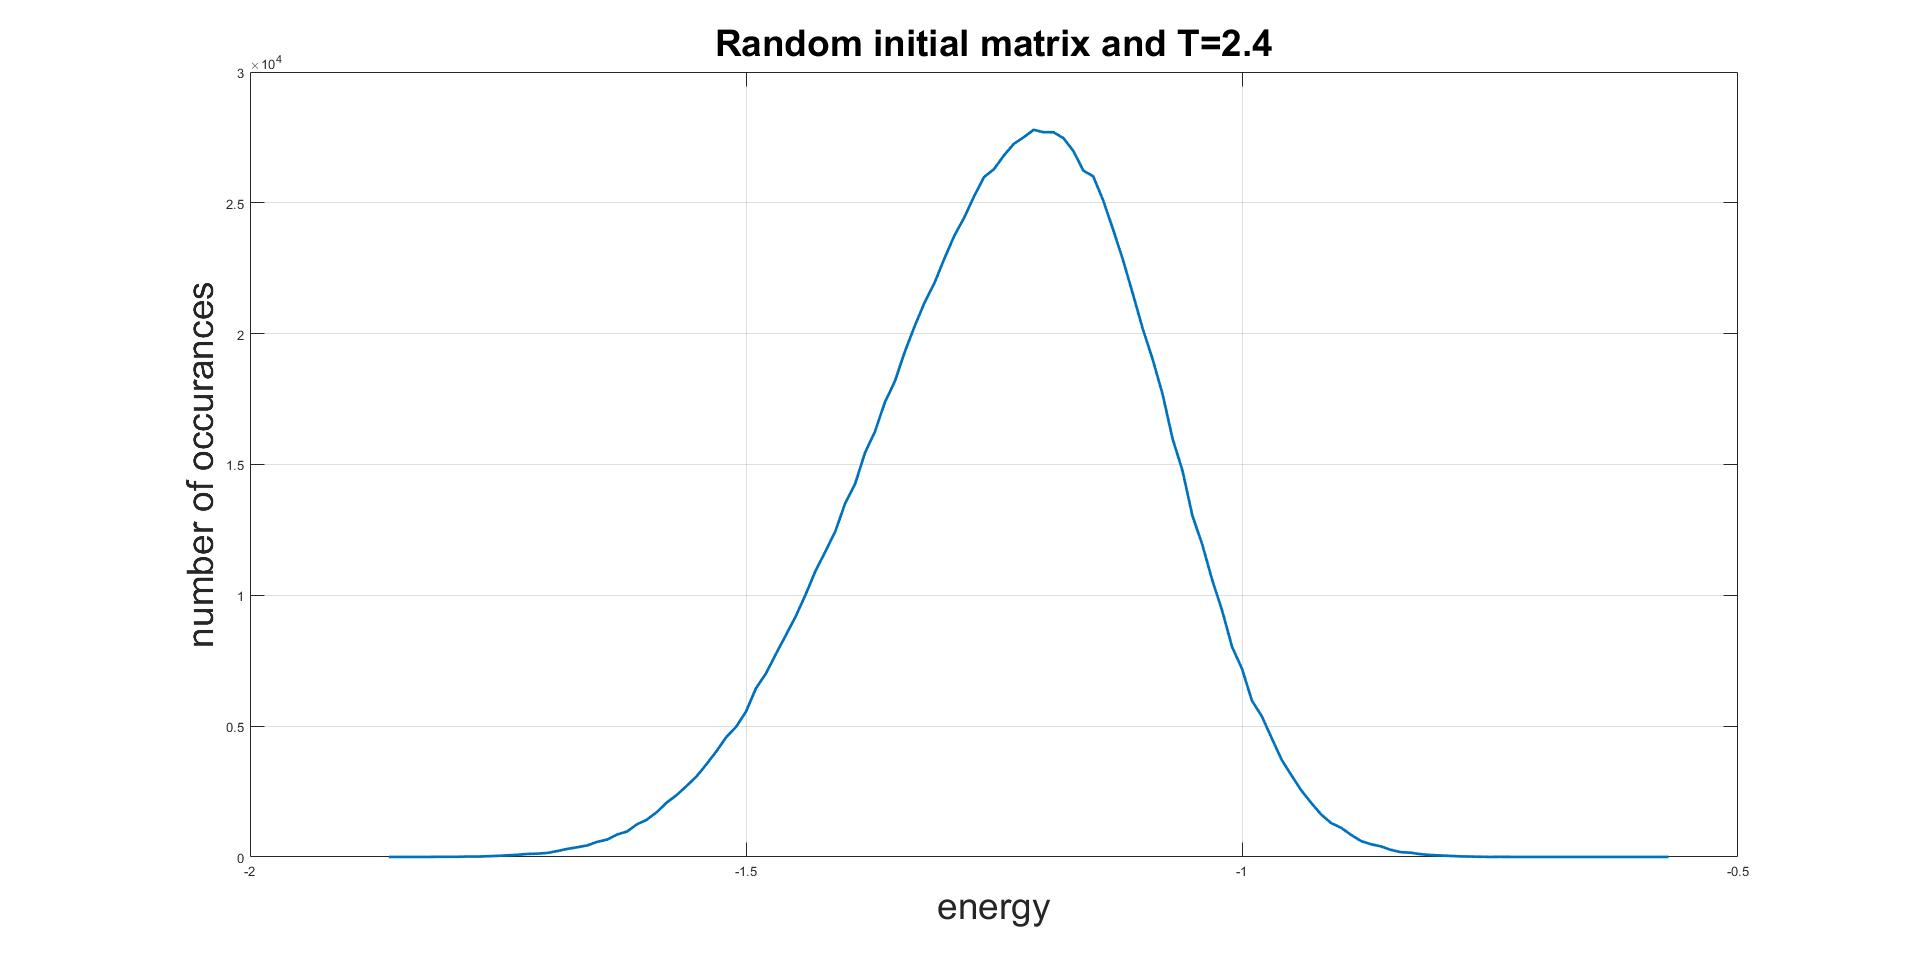
\includegraphics[scale=0.15]{OccurancesRandom.jpg}
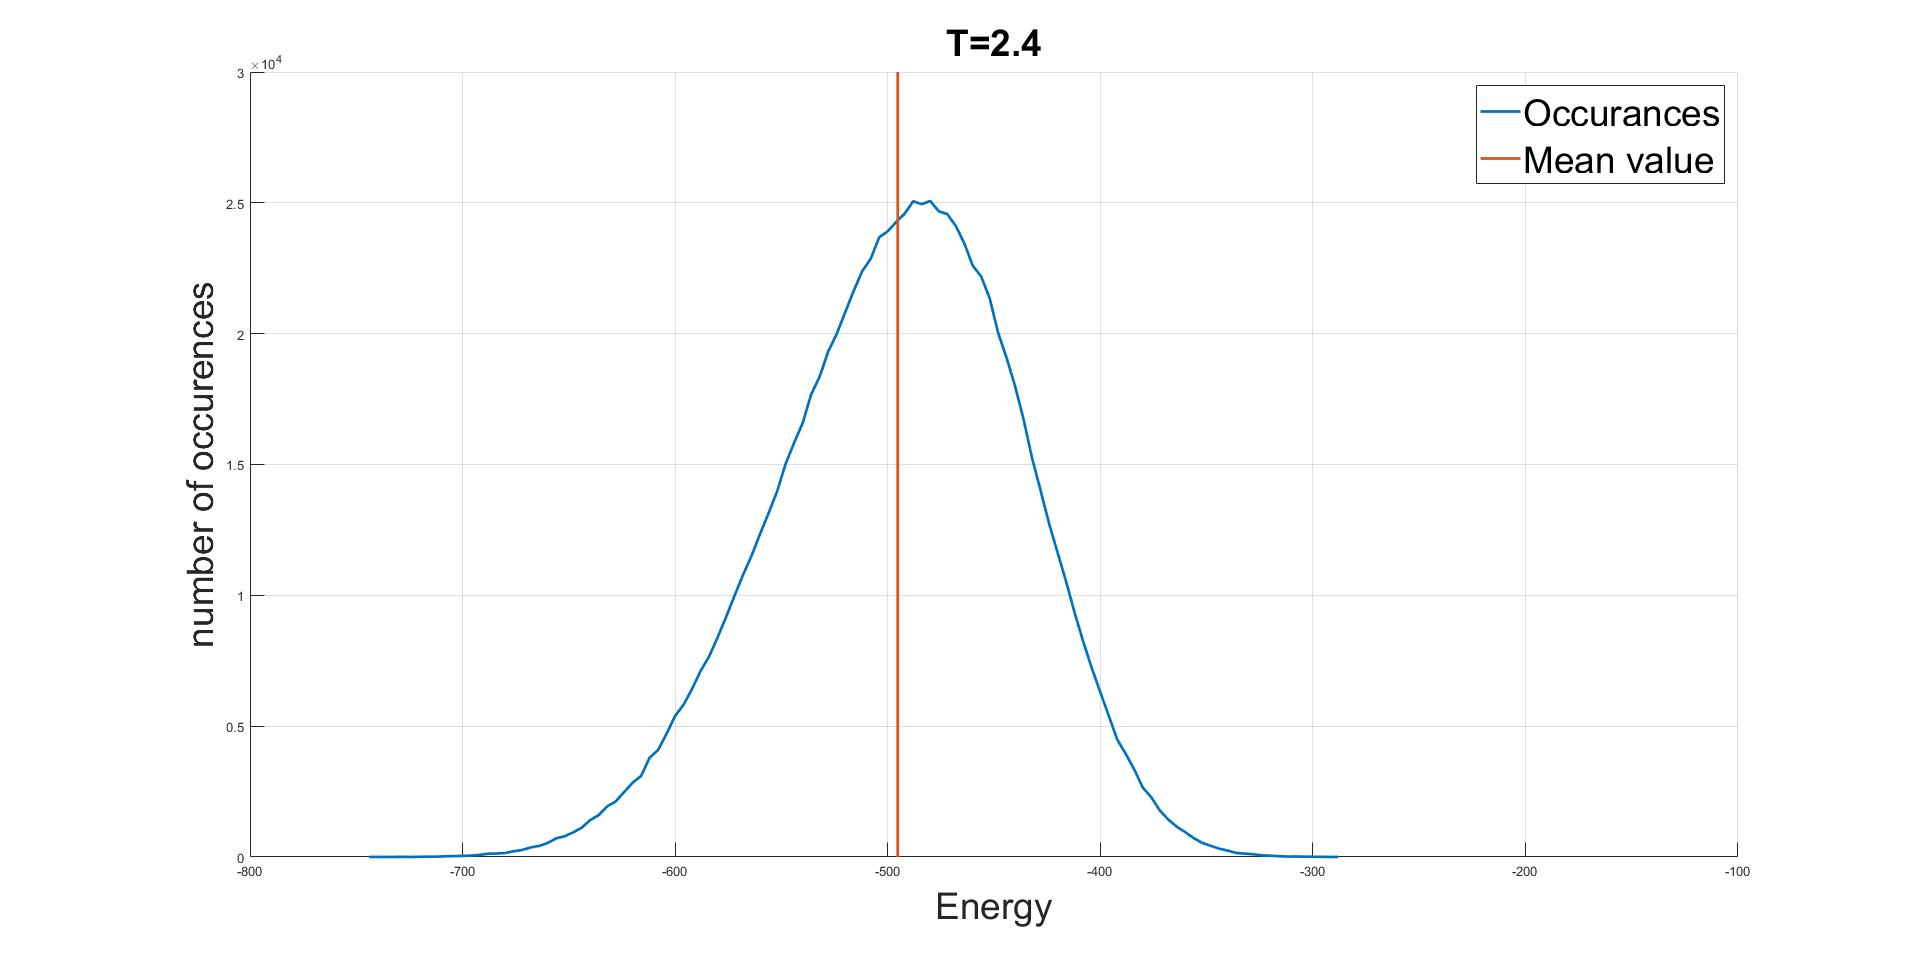
\includegraphics[scale=0.15]{OccurancesUp.jpg}
}
\caption{Occurances of different energies for a random initial matrix and an ordered initial matrix.}
\label{fig:ProbBoth}
\end{figure}


\newpage
\begin{tabular}{|l|c|}
\hline
  Temperature & Variance\\
\hline
  T=1.0 & 10.1076\\
\hline
  T=1.25 & 52.9558\\
\hline
  T=1.50 & 181.261\\
\hline
  T=1.75 & 478.219\\
\hline
  T=2.0 & 1157.08\\
\hline 
  T=2.25 & 3145.36\\
\hline 
  T= 2.50 & 2479.22 \\
\hline 
  T=2.75 & 1690.69\\
\hline
  T=3.0 & 1445.91\\
\hline
\end{tabular}
\\
computed with $10^6$ cycles. 




\newpage
{\LARGE\bf
Discussion 
}










\newpage
{\LARGE\bf
Conclusion
}
















\newpage
{\LARGE\bf
Reference list
}
\end{document}